\documentclass[11pt]{article}

\renewcommand{\baselinestretch}{1.8}
%\deff{\setl}{\setlength}
%\setl{\textwidth}{17.4 truecm}
\setlength{\textwidth}{17.5 truecm}
%\setl{\textheight}{22.2 truecm}
\setlength{\textheight}{22.8 truecm}
%\voffset -1.8 truecm
\voffset -2.3 truecm
%\hoffset -2 truecm
\hoffset -2 truecm


\usepackage{graphicx}
\usepackage{amsmath}
\usepackage{epstopdf}
\usepackage{floatrow}
\usepackage[T1]{fontenc}

\usepackage[noadjust]{cite}
\usepackage{filecontents}

\floatsetup[table]{capposition=top}

%\usepackage[]{subfig}
%\usepackage[font=small,format=plain,up]{caption}
\usepackage{cite}
\usepackage{floatrow}
\usepackage{fix-cm}
\newtheorem{theorem}{Theorem}
\makeatletter
\newcommand{\Rmnum}[1]{\expandafter\@slowromancap\romannumeral #1@}
\makeatother
\renewcommand{\citedash}{--}    
\newtheorem{thm}{Theorem}


\date{}

\begin{document}
\title{{\fontsize{20}{20}\selectfont An Information-theoretic Framework for Opportunistic, Mobile Social Networks}}

% author names and affiliations
% use a multiple column layout for up to three different
% affiliations
%\author{\IEEEauthorblockN{Mai EL-Sherief, Tamer EL-Batt, Ahmed Zahran}
%\IEEEauthorblockA{Wireless Intelligent Networks Center (WINC)\\
%School of Communication and Information Technology, Nile University\\
%Email:{mai.sherief, telbatt, a.h.zahran@nileu.edu.eg}} }

\author{\large Mai ElSherief $^\dagger$ $^\star$, Tamer ElBatt$^\dagger$ $^\star$,  Ahmed Zahran $^\dagger$ $^\star$, Ahmed Helmy $^\ddagger$  \\ [.1in]
\thanks{This work was funded in part by a Google Faculty Research Award.}
\small  \begin{tabular}{c} $^\dagger$Wireless Intelligent Networks Center (WINC), Nile University, Smart Village, Egypt.\\
$^\star$Faculty of Engineering, Cairo University, Giza, Egypt.\\
$^\ddagger$The Department of Computer and Information Science and Engineering,
University of Florida, Gainesville, USA. \\
%email: ahmed.arafa@nileu.edu.eg, kseddik@aucegypt.edu, salatino@stanfordalumni.edu,  telbatt@ieee.org, amr.elsherif@ieee.org
\end{tabular} }

\maketitle

\begin{abstract}
\end{abstract}

\section{Knowledge Sharing in Opportunistic, Social Networks}
\indent
In this section, we shift our attention to the second part of the paper, namely the step 
of knowledge sharing between "similar users". In this part, we introduce a novel information-theoretic mathematical framework, establish fundamental limits and results, as opposed to designing knowledge sharing schemes and policies, which constitute an interesting topic of future research. This part lays the basis for comparing and assessing the merits of future knowledge sharing schemes in opportunistic social networks.

 
The second problem, we wish to address is to quantify the knowledge a user can extract from an encounter and its maximum value using Information theory tools. The use of theoretic tools to examine the behavior of networks is not new. Graph theory has been used a lot in the literature to predict and study social networks performance as in \cite{graph1}, \cite{graph2} and \cite{graph3}. However, the incorporation of Information theoretic tools in opportunistic mobile social networks hasn't been introduced yet.

In this paper and after quantitatively assessing the similarity between mobile users given non-temporal or temporal profiles, we wish to take a look and investigate the collective knowledge available in an similarity-based opportunistic network. Modelling the user as a random variable opens ample room for using Information theory tools to measure different knowledge levels in the network. Section 1 introduces the system model in which we build our investigation upon. We then take a look about different performance metrics used to assess different forwarding schemes. We then introduce the Information-theoretic framework used to study the system in hand. We define novel concepts such as Knowledge Gain per encounter, Knowledge Capacity and Overhead per encounter in Section 2 We then introduce two profile dissemination policies namely Mine Only and Mine Plus Others'. In Section 3, we investigate two network topologies: directly connected and indirectly connected topology. We model the users using the LiveLab \cite{data} data traces. We also investigate the previously mentioned topologies in a stationary scenario and using InfoCom 2005 \cite{infocom} mobility traces in a mobile scenario.

%%%%%%%%%%%%%%%%%%%%%%%Profile Structure & Management%%%%%%%%%%%%%%%%%%%%%%%%%%%%%%%
\section{Performance Metrics for Information Dissemination Policies}
\subsection{System Model}
The system model is basically a similarity-based network consisting of $M$ nodes. Each node has its own profile for interests and experiences represented in our system as a single PMF or multiple PMFs across the temporal dimension across different pre-defined categories. Each node also possess some \textit{information tips} e.g. a recommendation that a place is good, an interesting upcoming event, etc. that they can exchange with similar users to increase their knowledge.\\
\indent The $M$ nodes happened to meet opportunistically in a place e.g. super market, museum, club, etc. In this similarity-based network, the nodes don't exchange tips unless they are deemed similar. We measure the similarity between nodes by the classic cosine similarity or a variation of this metric between the PMFs of the users. We also assume that the probabilistic characteristics of the information tips that a user has are similar to the probabilistic characteristics of the user's behaviour captured via his/her interests and experiences (same first and higher order PMFs).\\
\indent
For this model, and using different dissemination policies we wish to assess quantitatively the performance of the different forwarding policies through different metrics that we will discuss in detail shortly.
An effective dissemination policy would disseminate one's tips to all similar nodes in the network without incurring a large overhead given energy constraints.
\subsection{Performance Metrics}
\begin{itemize}
\item Delivery Percentage: If there are $k$ similar users to a certain user, an optimal dissemination policy would disseminate one's tips to all the $k$ users. In general the delivery percentage is defined as the number of similar users reached $k\prime$ out of the $k$ similar users. We will show later that this resembles all users achieving their Knowledge Capacity.
\item Average cost: the cost in our context is the average hop count the tip takes to reach the destination.
\item Forwarding Efficiency: is defined as dividing the delivery percentage by the average cost.
\item Knowledge Gain: will be discussed in detail in the next section.
In the next section, we will introduce the Information-theoretic framework that will enable us to model most of the aforementioned metrics in an Information-theoretic fashion. For the next sections we will assume a mobile user $X$ is a random variable that has a discrete probability mass function (PMF). It is noted that modelling the mobile user as a random variable opens ample room for the use of Information theory as atool in characterizing notions such as Knowledge Gain, Knowledge Capacity and Overhead as follows.
\end{itemize}
\section{Knowledge Gain and Knowledge Capacity}
In this section we introduce two notions that will be help us in the theoretical analysis of the performance of different information dissemination policies.
\begin{itemize}
\item Knowledge Capacity for a given user (KC): defined as an upper bound on the maximum amount of new information that a user can extract from the similar users in a given network.
\item Knowledge Gain for a given user (KG): defined as the amount of new information that a user extracted from the similar users in a given network via a specific dissemination policy. Axiomatically, the Knowledge Gain is always less than or equal to the Knowledge Capacity.
\end{itemize}
Since our model is probabilistic in nature (i.e the users' profiles are represented by PMFs), we use Information theory tools as one way to quantify both aforementioned notions.
\subsection{Knowledge Gain per Encounter}
Using our Assumption stated earlier that the probabilistic characteristics of the tips are the same as the probabilistic characteristics as his/her behaviour. We can use the information-theoretic entropy to help us quantify both Knowledge Gain and Knowledge Capacity.\\
If we have two users $X$ and $Y$ who happen to opportunistically meet according to the similarity based opportunistic network that was described earlier and are deemed similar, they can now exchange tips.
Using Information theory, we can quantify three important parts as indicated in Fig. ~\ref{fig:KGEncounter}
\begin{itemize}
\item A part of the tips that user $X$ possesses and $Y$ doesn't possess.
\item A part of the tips that user $X$ possesses and $Y$ doesn't possess.
\item A part of the tips that both user $X$ possesses and $Y$ possesses also.
\end{itemize}
If $X$ and $Y$ are deemed similar and they exchange tips. From the point of view of $Y$, the new information he/she gained is the first part mentioned earlier. This part is $H(X|Y)$ i.e. the Entropy (uncertainty/information content) of user $X$ given $Y$. So, the Knowledge Gain (KG) for user $Y$ in this case is $H(X|Y)$. Along the same lines, for user $X$, $KG=H(Y|X)$.
Using some basic definitions from Information theory, we can rewrite the KG for user $X$ as $H(X,Y)-H(X)$. This can be directly interpreted as the amount of joint info that both $X$ and $Y$ have minus the amount of info that $X$ has.
The third part $I(X;Y)$ is considered to be the overhead of the exchange since it is considered part of the resources that don't contribute to the benefit of $X$ or to the benefit of $Y$.

\begin{figure}[!tp]
  \centering
    \includegraphics[width=10cm ,height=7cm]{figures_png/vennSimple}
    \caption{Characterizing Knowledge Gain and Overhead for X and Y.}\label{fig:KGEncounter}
    \end{figure}
 
\subsection{Knowledge Capacity}
Extending the insights that we formed about the KG quantity from the last subsection, we can now generalize the insights to get the general form for the Knowledge Capacity for a single user in a similarity-based opportunistic network of $M$ users.
We can define the Knowledge Capacity(KC) for a single user $X_1$ as follows,
\begin{equation}
		KC(X_1) = H(X_1, X_2, X_3, ......, X_M) - H(X_1)
\end{equation}

		$ | X_2, X_3, ......, X_M$ are similar to $X_1$
which is directly equivalent to without loss of generality,
$$H(X_2|X_1) + H(X_3|X_2,X_1) + .....+ H(X_M|X_{M-1}, ......, X_1)$$
$ | X_2, X_3, ......, X_M$ are similar to $X_1$.
This definition means that the maximum amount of information that user $X_1$ can extract from the network is simply the joint information that all users have removing any duplicates which is represented by this term  $H(X_1, X_2, X_3, ......, X_M)$ minus the amount of information that user $X_1$ possess which is represented by $H(X_1)$.\\

Using these information theoretic tools and defining two basic information dissemination policies, we delve into different network configurations and attempt to apply the aforementioned definitions on them in order to further study them.
\subsection{Information Dissemination Policies}
Throughout the network model that we explained earlier, we can think of two extreme tips' exchange policies per encounter. Of course as explained earlier, the tips exchange occur only if the two users are deemed similar.
\begin{itemize}
\item Forward My Tips Only: or "Forward Mine Only" In this policy if the two users are similar, each one sends his/her own tips only.
\item Forward My Tips and others: or "Forward Mine Plus Others'" In this policy if the two users are similar, each one sends his/her tips and the tips that he/she acquired from previous encounters.
\end{itemize}
Of course one can think of other policies or derivative policies from the previous two policies. For example we could have a policy of forwarding own tips in addition to forwarding one only from the other's tips or two or three. Another hybrid policy would be forward My Tips only with probability $p$ and forward mine plus others with probability $1-p$.
Our main focus in this work is to analyse the network dynamics for the two main dissemination policies: Forward Mine Only and Forward Mine Plus Others.
\section{Similarity Based Network Analysis for Different Scenarios}
The network model described earlier may/may not incorporate a Mobility component. We need to study both stationary and mobile models since the nodes may be stationary or moving around in the network area. We will study both directly and indirectly connected networks as the proximity/topology of the nodes play an important role since the communication that occurs here is point to point. For simplicity here, we will assume all the nodes in the network are mutually similar to focus on the Knowledge related concepts.
\subsection{Stationary Similarity-based Opportunistic Network}

\subsubsection{Data used for Experimentation}
For the Stationary Similarity-based Opportunistic networks and modeling the user as a Random Variable, we will be conducting our experiments using LiveLab data \cite{data} described earlier. The network consists of $20$ nodes;  $B00$, $B02$, $B03$,
$B04$, $B05$, $B06$, $B07$, $B08$, $B09$, $B10$, $B11$, $D00$, $D01$, $D02$, $D03$, $D04$, $D05$, $D06$, $D07$ and $D08$. We shall investigate the cumulative knowledge gain after each encounter and whether the gain will reach capacity or not and how many encounters shall it take to reach capacity.
\subsubsection{ Stationary Directly Connected (Single Hop) Network:}

In this kind of network, all nodes are in the same communication range of each other. Each node is a single hop away from other nodes, thus the name "Single Hop Network".
For this network we can prove that the Knowledge Gain will reach the Knowledge Capacity.
Simply, since all nodes are in the same communication range of all other nodes, any node will be able to encounter any other node and extract its information, and if we assume that all nodes are mutually similar, the additive knowledge Gain will simply yield the Knowledge Capacity and this can be shown shortly.\\

\begin{itemize}
\item{Stationary Directly Connected (Single Hop) Network - Forward Mine Only:}
in this network all nodes are in each others' range and if two users are deemed similar, each user exchanges only his/her tips.
We now present a theorem and its proof suggesting that all nodes can achieve knowledge capacity.

\begin{theorem}
For a Stationary Directly Connected (Single Hop) Network, any node can achieve Knowledge Capacity using Mine Only forwarding policy.\\

\end{theorem}

%\begin{proof}
\textit{Proof:}\\
Without loss of generality, we will assume that node $X_1$ will encounter other nodes in the network in an increasing order of node id and we assume a Forward Mine Only Policy as in Fig.~\ref{SSHPNet}. So, the cumulative knowledge gain for node $X_1$ $KG(X_1)$ according to meeting nodes $X_2, X_3, X_4,...., X_M$ will be $$H(X_2|X_1) + H(X_3|X_2,X_1) + .....+ H(X_M|X_{M-1}, ......, X_1)$$ and this summation is itself $$H(X_1, X_2, X_3, ......, X_M) - H(X_1)= KC(X_1)$$. The same can also be applied to any other node and along the same lines we can prove that it can achieve its knowledge capacity.\\
\begin{figure}[!tp]
\centering
    \includegraphics[width=10cm ,height=7cm]{figures_png/SSHPNet}
    \caption{$X_1$ encounters enumerated.}\label{fig:KGEncounter}
    \label{SSHPNet}
\end{figure}

%\end{proof}
Of course if there is at least one node isolated from the rest of the network that has at least one new tip (piece of information), it can be easily shown that $KG(X_1) \leq KC(X_1)$.\\
\begin{theorem}
If there is at least one node isolated from the rest of the a directly connected network that has at least one new tip (piece of information), $KG(X_1) \leq KC(X_1)$.\\
\end{theorem}
\textit{Proof:}\\
Without loss of generality, we will assume that node $X_1$ will encounter other nodes in the network in an increasing order of node id and we assume a Forward Mine Only Policy. If node $X_M$ is isolated and can't be reached. So, the cumulative knowledge gain for node $X_1$, $KG(X_1)$, according to meeting nodes $X_2, X_3, X_4,...., X_{M-1}$ will be $$H(X_2|X_1) + H(X_3|X_2,X_1) + .....+ H(X_{M-1}|X_{M-2}, ......, X_1)$$ and this summation is missing the last term $H(X_M|X_{M-1}, ......, X_1)$ and since the entropy value is always greater than or equal zero so 
$KG(X_1) <  KC(X_1) $.\\

\indent One of the important issues here is how fast any user can achieve his/her Knowledge Capacity. In this work we will measure how fast this occurs by computing the Number of Exchanges that a user needs to perform to attain the capacity.
To illustrate more, if for this stationary similarity-based opportunistic network each node uses a Forward My Tips Only as a dissemination policy assuming each node has at least one piece of information to contribute to the network, then the number of exchanges needed for each node to attain the capacity is $N-1$ exchanges which is $O(N)$ assuming of course that each node has at least one new tip to contribute to the knowledge of the network .\\
\item{Stationary Directly Connected (Single Hop) Network - Forward Mine Plus Others':}
in this network all nodes are in each others' range and if two users are deemed similar, each user exchanges his/her tips and the tips he/she has extracted from previous encounters. We model previous tips by subscript $p$.

\indent For the Stationary Directly Connected (Single Hop) network, and using Mine Plus Others' forwarding scheme, we can also show that any node can achieve the Knowledge Capacity.\\
\textit{Example:}In a network of $4$ nodes ($X_1, X_2, X_3, X_4$), if we use a Mine Only forwarding scheme, $X_1$ will have to make $3$ encounters with $X_2, X_3$ and $X_4$ to reach its Knowledge Capacity. If we use a Mine Plus Others' forwarding scheme as shown in Fig. $X_1$ will reach the capacity in $2$ encounters.\\
\begin{theorem}
For a Stationary Directly Connected (Single Hop) Network, any node can achieve Knowledge Capacity using Mine Plus Others' forwarding policy.
\end{theorem}

%\begin{proof}
\textit{Proof:}\\
Without loss of generality, we will assume that node $X_1$ will encounter other nodes in the network in an increasing order of node id and we assume a Forward Mine Plus Others' policy. So, the cumulative knowledge gain for node $1$ $KG(X_1)$ according to meeting nodes $2, 3, 4,...., M$ will be $H(X_2,|X_1) + H(X_3, \vec{X_{3p}}|X_2,X_1) + H(X_4, \vec{X_{4p}}|X_3, \vec{X_{3p}}, X_2,X_1)+.....+ H(X_M, \vec{X_{Mp}}|X_{M-1}, \vec{X_{(M-1)p}} ,......, X_1)$ and this summation is itself $$H(X_1, X_2, X_3, ......, X_M) - H(X_1)= KC(X_1)$$ where $\vec{X_Np}$ stands for the previous encounters of Node $N$.\\
Of course once the right hand side of the given sign has the full list of the nodes in the network, the added gain will be zero and the node will have reached its Knowledge Capacity. That is why the Mine Plus Others' policy can attain the capacity faster due to the terms that contain the previous encounters. Of course this doesn't come at a free cost. It can be proved that the overhead of using a Mine Plus Others' policy greater than or equal the Mine Only Policy.\\
\begin{theorem}
The overhead of using a Mine Plus Others' policy is greater than or equal the overhead of using a Mine Only Policy.
\end{theorem}
\textit{Proof:}\\
Let's assume that two users $X$ and $Y$ encounter each other. Let us denote the vector of previous encounters for $X$ by $\vec{X_p}$ and the previous encounters for $Y$ by $\vec{Y_p}$.\\
For the Forward Mine Only policy the Overhead for user $X$ is the mutual information between what he/she has and what he/she expects from user $Y$ which is 
\begin{equation}
I(X,\vec{X_p};Y).
\label{overheadX}
\end{equation}
Similarly the overhead from the perspective of user $Y$ is $I(Y,\vec{Y_p};X)$.\\
For the Forward Mine Plus Others' scheme the overhead from the perspective of user $X$ is the same from the perspective of user $Y$ which is
\begin{equation} 
I(X,\vec{X_p};Y, \vec{Y_p}).
\label{overheadXY}
\end{equation}
As we know from Information Theory the mutual information between two users $A$ and $B$ can be re-written as
\begin{equation} 
I(A;B)=H(A) + H(B) - H(A,B).
\label{mutInfoEqn}
\end{equation}
Applying ~\eqref{mutInfoEqn} on the term in ~\eqref{overheadXY}, we get
\begin{equation}
I(X,\vec{X_p};Y,\vec{Y_p})= H(X,\vec{X_p})+H(Y,\vec{Y_p})-H(X,\vec{X_p},Y,\vec{Y_p}).
\label{Eqn.3}
\end{equation}
Applying ~\eqref{mutInfoEqn} on the term in ~\eqref{overheadX}, we get
\begin{equation}
I(X,\vec{X_p};Y)= H(X,\vec{X_p})+H(Y)-H(X,\vec{X_p},Y).
\label{Eqn.4}
\end{equation}
By Subtracting Equation ~\eqref{Eqn.4} from ~\eqref{Eqn.3} we get 
\begin{equation}
H(Y,\vec{Y_p})-H(Y)-H(X,\vec{X_p},Y,\vec{Y_p})+H(X,\vec{X_p},Y).
\label{Eqn.5}
\end{equation}
Since $H(\vec{A},\vec{B}) = H(\vec{A}) + H(\vec{B}|\vec{A}) = H(\vec{B}) + H(\vec{A}|\vec{B}) $, ~\eqref{Eqn.5} could be written as
\begin{equation}
H(Y)+H(\vec{Y_p}|Y)-H(Y)-[H(X,\vec{X_p},Y) + H(\vec{Y_p}|X,\vec{X_p},Y)] + H(X,\vec{X_p},Y)
\end{equation}
which reduces to 
\begin{equation}
H(\vec{Y_p}|Y)- H(\vec{Y_p}|X,\vec{X_p},Y)
\label{lasteqn}
\end{equation}
and we know from Information theory that conditioning can't increase the entropy so $H(\vec{Y_p}|X,\vec{X_p},Y) \leq H(\vec{Y_p}|Y)$ making ~\eqref{lasteqn} greater than or equal zero which proves that the overhead of the Mine Plus Others' Policy is greater than or equal the overhead of the Mine Only Policy which concludes our Proof.

\end{itemize}
\textit{Example: }As an example on speeding up the achievability, let's envision a network of $4$ users: $X_1, X_2, X_3, X_4$ as shown in Fig.~\ref{fig:SSHP(MO1)}. As shown in the figures Knowledge Before the Exchange (BFE) and Knowledge After the Exchange (BAE). We can see from Fig.~\ref{fig:SSHP(MO2)} that all nodes have reached the capacity after $2$ encounters only instead of $M-1$ encounters for the Forward Mine Only Policy.
\begin{figure}[!bp]
\centering
    \includegraphics[width=10cm ,height=7cm]{figures_png/SSHP(MO1)}
    \caption{A scenario for encounters (First Step).}\label{fig:SSHP(MO1)}
    \label{SSHP(MO1)}
\end{figure}
\begin{figure}[!bp]
\centering
    \includegraphics[width=10cm ,height=7cm]{figures_png/SSHP(MO2)}
    \caption{A scenario for encounters (Second Step).}\label{fig:SSHP(MO2)}
    \label{SSHP(MO2)}
\end{figure}


%On the other hand, if we each node uses a Forward My Tips and others dissemination policy and if we assume that the system of the nodes will be exchanging tips for a while before a new node enters the network environment, then we have two extreme cases as follows.\\
%In the best case, where the new entering node named $X$ meets a node that has gathered all the tips in the system named $Y$, then the number of exchanges that $X$ needs to attain capacity is one, hence a complexity of $O(1)$.\\
%On the other hand, the worst case scenario is simply when no enough exchanges are done before node $X$ enters the system and this leads to the Mine plus others scheme falling back to the Mine Only scheme and the number of exchanges needed by $X$ to attain capacity will be $O(N)$.
\subsubsection{Stationary Indirectly Connected Network:} in this kind of network, not all nodes are in the same communication range of each other. If we take node $X_1$ for example, then in this kind of network it will have a subset of the $M$ nodes, say $N$ where $N<M$, in the same communication range or one hop away and the other $M-N$ nodes not reachable by $X_1$.\\
Here the information dissemination policy plays an important role in whether or not a node attains the Knowledge Capacity.
\begin{itemize}
\item{Stationary Indirectly Connected (Multi-Hop) Network - Forward Mine Only:}
If the dissemination policy used in this network shown in Fig.~\ref{SMHPNet} is Forward Mine Only, then we can see that the Knowledge Gain achieved by node $X_1$ is limited by $N$ i.e., the neighbourhood size of node $X_1$. So, since $N$ is strictly less than $M$ the Knowledge Gain will be less than the Knowledge Capacity.\\
\textit{Proof:}\\
Without loss of generality, we will assume that node $X_1$ will encounter other nodes in the network in an increasing order of node id and we assume a Forward Mine Only Policy. The cumulative knowledge gain for node $X_1$, $KG(X_1)$, according to meeting nodes $X_2, X_3, X_4,...., X_{N}$ will be $$H(X_2|X_1) + H(X_3|X_2,X_1) + .....+ H(X_{N}|X_{N-1}, ......, X_1)$$ and this summation is missing the terms $H(X_{N+1}|X_{N}, ......, X_1)$ till $H(X_{M}|X_{M-1}, ......, X_1)$ and since these terms are entropy terms whose values are always greater than or equal zero so $KG(X_1) <  KC(X_1)$.\\
The situation differs for example for any node that has all nodes in its range i.e., $N=M$. For this node, capacity will be achieved (all missing terms from the last proof will be added and the gain reaches capacity). We will show later that if the network incorporates a mobility component, capacity could be achieved for all nodes even if $N<M$.\\

\begin{figure}[!tp]
\centering
    \includegraphics[width=10cm ,height=7cm]{figures_png/SMHP(MO)}
    \caption{Stationary Indirectly Connected (Multi-Hop) Network.}\label{fig:SMHP(MO)}
    \label{SMHPNet}
\end{figure}
%==============================================================================================================
\item{Stationary Indirectly Connected (Multi Hop) Network - Forward Mine Plus Others':}
For the same network depicted in Fig.~\ref{SMHPNet}, we now study this network using a Forward Mine Plus Others' policy. If we assume multiple encounters with the same node is allowed and the neighbouring nodes for $X_1$ collected the knowledge of non-neighbouring nodes for $X_1$, then $X_1$ can attain its knowledge capacity. We now present this in the next theorem.
\begin{theorem}
For a given indirectly connected (multi-hop) network, any node can achieve Knowledge Capacity using Mine Plus Others' forwarding policy.
\end{theorem}
\textit{Proof:}
Without loss of generality, we will assume that node $X_1$ will encounter other nodes in the network in an increasing order of node id and we assume a Forward Mine Plus policy. So, the cumulative knowledge gain for node $1$ $KG(X_1)$ according to meeting nodes $2, 3, 4,...., M$ will be $H(X_2,|X_1) + H(X_3, X_{3p}|X_2,X_1) + H(X_4, X_{4p}|X_3, X_{3p}, X_2,X_1)+.....+ H(X_N, X_{Np}|X_{N-1}, X_{(N-1)p} ,......, X_1)$. If all the previous encounters constitute $X_{N+1}, X_{N+2}, ......, X_M$, then the cumulative knowledge gain will yield $$H(X_1, X_2, X_3, ......, X_M) - H(X_1)= KC(X_1)$$ where $X_Ip$ stands for the previous encounters of Node $I$. If all the previous encounters don't constitute $X_{N+1}, X_{N+2}, ......, X_M$, then we need to allow $X_1$ to revisit the nodes that it has already visited to acquire from them the missing knowledge of the nodes not in its range until it eventually reaches capacity. Of course once the right hand side of the given sign has the full list of the nodes in the network, the added gain will be zero and the node will have reached its Knowledge Capacity.\\
\end{itemize}

%On the contrary, if the dissemination policy used in this network is Forward Mine Plus Others we can find best and worst cases scenarios.
%The best case for this situation happens when the $N$ neighbouring nodes have the knowledge (tips) of the non-neighbouring nodes. If that is the case and through using the Mine plus others policy, $X$ could attain the Knowledge Capacity.
%The worst case for this situation happens when the $M-N$ non neighbouring nodes for $X$ can't be reached by the $N$ neighbouring nodes and thus this case falls back to the Mine Only strategy in the last paragraph.
%The average case naturally happens when some of the non-neighbouring nodes are achievable and some aren't and in this case also $X$ can't attain Knowledge Capacity as well.

\subsubsection{LiveLab Results for Stationary Similarity-based Opportunistic Network }
After describing the different topologies for the similarity-based Opportunistic Network under investigation, we now present the results after incorporating $20$ LiveLab users as the nodes for the network. For our investigation and to calculate the capacity and the knowledge gain for every encounter, we implement an multi-threaded algorithm that computes the joint PMF for the users under investigation taking into account a period of six months from September 2010 to February 2011. We monitor the users' activities categorized under $24$ categories second by second for the six months and record what they are doing simultaneously and after that we divide by the total duration of the six months to get a PMF. We present the results for the cumulative knowledge gain across the encounter number as follows.
%===========================================================================================================
\begin{itemize}
\item Results for Stationary Directly Connected (Single-Hop)- Mine Only Network:
For this kind of network, any node can achieve the knowledge capacity in $19$ exchanges. This is shown in Fig.~\ref{fig:B00_SSHOP)} for user $B00$, in Fig.~\ref{fig:B02_SSHOP)} for user $B02$ and for user $D00$ in Fig.~\ref{fig:D00_SSHOP)}.

\begin{figure}[!tp]
\centering
    \includegraphics[width=15cm ,height=8cm]{figures_eps/B00_SSHOP}
    \caption{Cumulative Knowledge Gain for user B00 in a stationary directly connected network (Forward Mine Only).}\label{fig:B00_SSHOP)}
    \end{figure}
    \begin{figure}[!tp]
\centering
    \includegraphics[width=15cm ,height=8cm]{figures_eps/B02_SSHOP}
    \caption{Cumulative Knowledge Gain for user B02 in a stationary directly connected network (Forward Mine Only).}\label{fig:B02_SSHOP)}
    \end{figure}
    \begin{figure}[!tp]
\centering
    \includegraphics[width=15cm ,height=8cm]{figures_eps/D00_SSHOP}
    \caption{Cumulative Knowledge Gain for user D00 in a stationary directly connected network (Forward Mine Only).}\label{fig:D00_SSHOP)}
    \end{figure}
%================================================================================================================
\item Results for Stationary Directly Connected (Single-Hop)- Mine Plus Others' Network:
For this kind of network we can notice that all nodes achieve capacity as in the Mine Only case but after less encounters. This is shown for users $B00$, $B04$ and $D03$ in Fig.~\ref{fig:B00_SSHOP(MO)}, ~\ref{fig:B04_SSHOP(MO))} and ~\ref{fig:D03_SSHOP(MO))} respectively.


 \begin{figure}[!bp]
\centering
    \includegraphics[width=15cm ,height=8cm]{figures_eps/B00_SSHOP_MO.eps}
    \caption{Cumulative Knowledge Gain for user B00 in a stationary directly connected network (Forward Mine Plus Others').}\label{fig:B00_SSHOP(MO)}
    \end{figure}
    
     \begin{figure}[!bp]
\centering
    \includegraphics[width=15cm ,height=8cm]{figures_eps/B04_SSHOP_MO.eps}
    \caption{Cumulative Knowledge Gain for user D00 in a stationary directly connected network (Forward Mine Plus Others').}\label{fig:B04_SSHOP(MO))}
    \end{figure}
    
     \begin{figure}[!bp]
\centering
    \includegraphics[width=15cm ,height=8cm]{figures_eps/D03_SSHOP_MO.eps}
    \caption{Cumulative Knowledge Gain for user D00 in a stationary directly connected network (Forward Mine Plus Others').}\label{fig:D03_SSHOP(MO))}
    \end{figure}
%=================================================================================================================
\item Results for Stationary Indirectly Connected (Multi-Hop)- Mine Only Network: 

For this kind of network, any node is limited in achieving the capacity by the neighbourhood size. For instance, user $B00$ had only $B03$, $B05$, $B09$, $B11$, $B07$, $D01$, $D03$, $D05$ in its range, so it didn't reach the capacity as shown in Fig. ~\ref{fig:B00_SMHOP)}.
The same applies for users $B06$ and $D00$ in which their neighbourhood contained only a subset of all $M$ users so they didn't reach their full capacities as shown in Fig.~\ref{fig:B06_SMHOP)} and Fig.~\ref{fig:D00_SMHOP)} respectively.
\begin{figure}[!bp]
\centering
 \includegraphics[width=15cm ,height=8cm]{figures_eps/B00_SMHOP}
    \caption{Cumulative Knowledge Gain for user B00 in a stationary indirectly connected network (Forward Mine Only).}\label{fig:B00_SMHOP)}
    \end{figure} 
    \begin{figure}[!bp]
	\centering
     \includegraphics[width=15cm ,height=8cm]{figures_eps/B06_SMHOP}
    \caption{Cumulative Knowledge Gain for user B06 in a stationary indirectly connected network (Forward Mine Only).}\label{fig:B06_SMHOP)}
    \end{figure}
    
    \begin{figure}[!bp]
	\centering
     \includegraphics[width=15cm ,height=8cm]{figures_eps/D00_SMHOP}
    \caption{Cumulative Knowledge Gain for user D00 in a stationary indirectly connected network (Forward Mine Only).}\label{fig:D00_SMHOP)}
    \end{figure}
    
\item Results for Stationary Indirectly Connected (Multi-Hop)- Mine Plus Others' Network: 
We expect from this kind of network that Mine Plus Others' forwarding policy can fight node location limitation and nodes could reach capacity. The results for this network is based on a three-layer topology. The first layer contains node $B00$, the second layer contains ten nodes and the third layer contains nine nodes. Each layer could only encounter nodes in the directly lower layer or directly upper layer only. The results for this kind of network for users $B00$, $B06$ and $D00$ are depicted in Fig.~\ref{fig:B00_SMHOP_MO)}, ~\ref{fig:B06_SMHOP_MO)} and ~\ref{fig:D00_SMHOP_MO)} respectively.

  \begin{figure}[!bp]
	\centering
     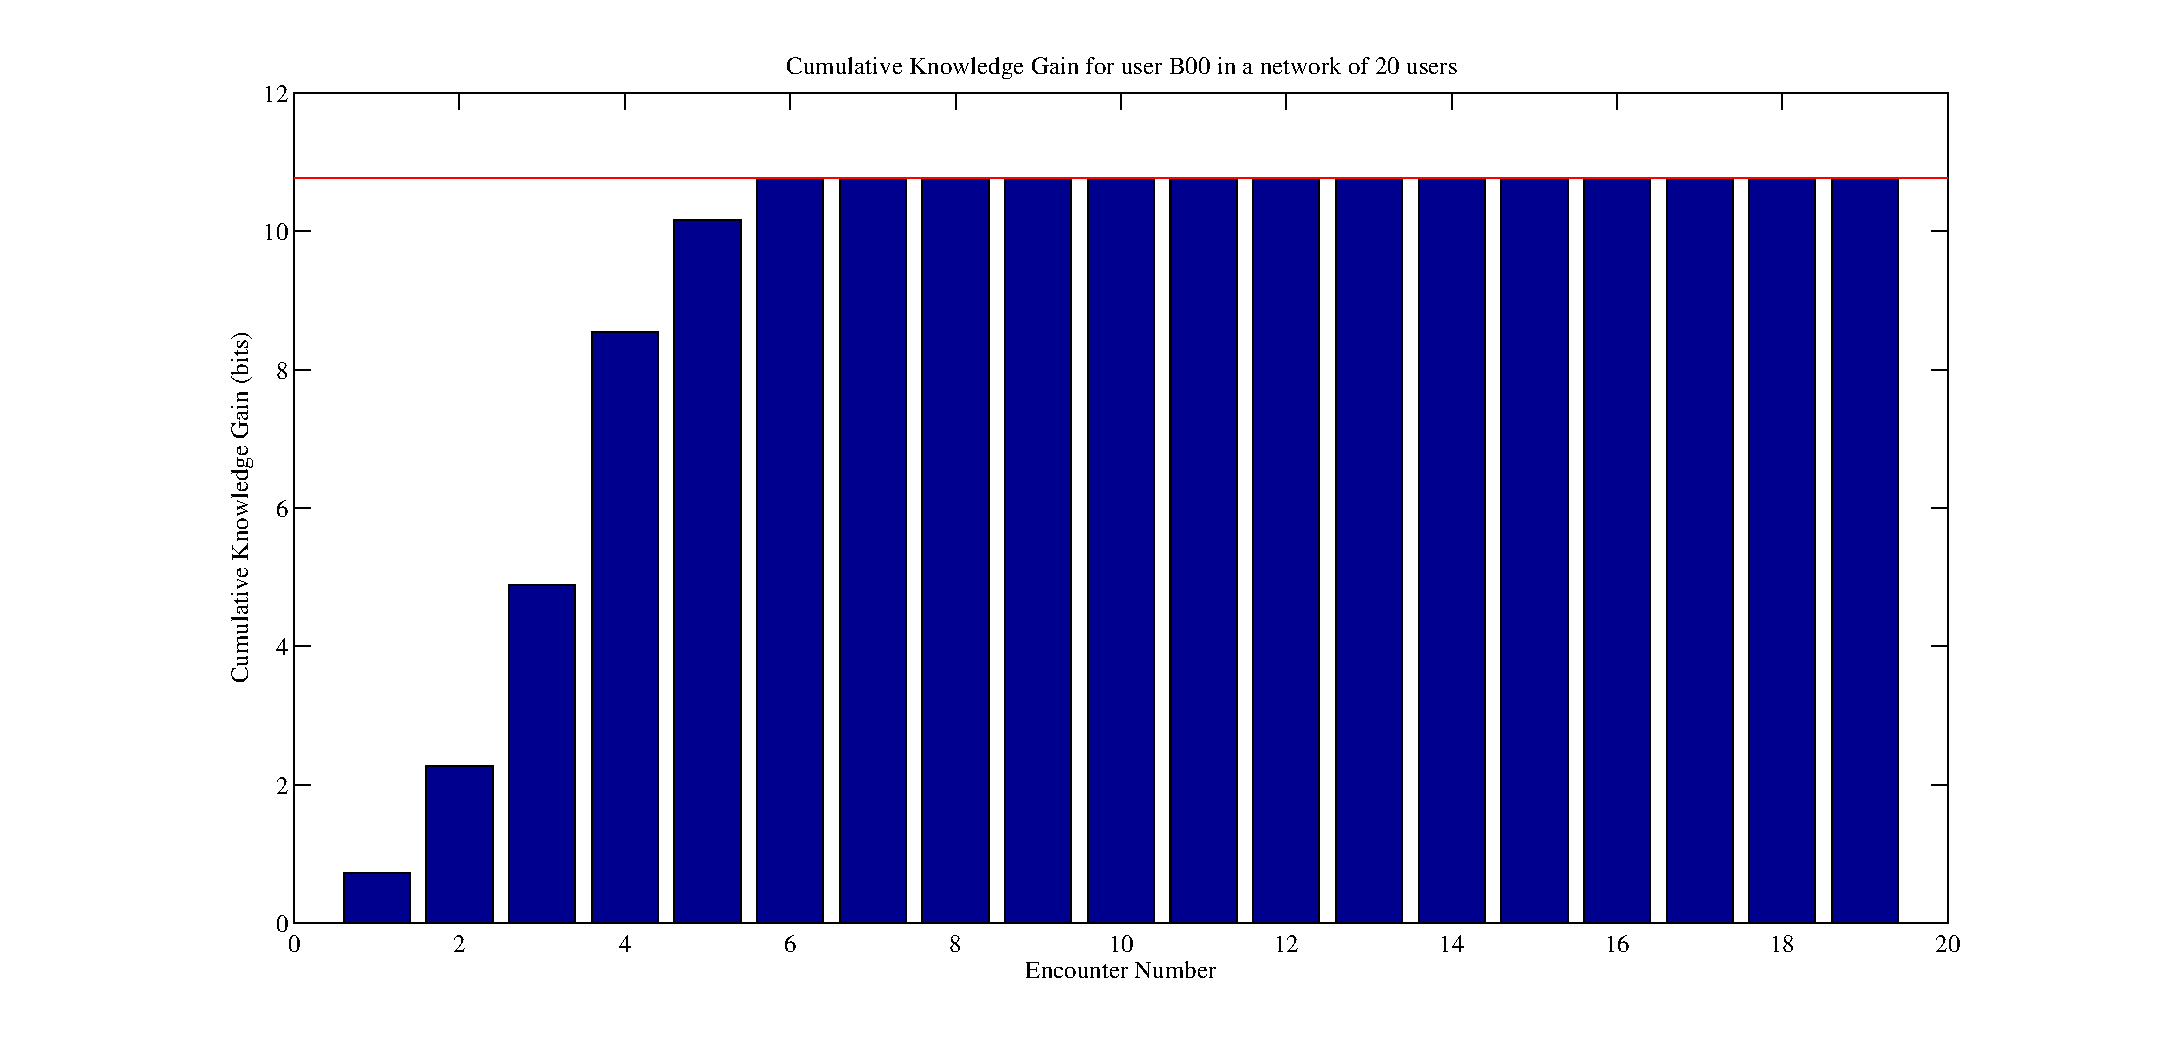
\includegraphics[width=15cm ,height=8cm]{figures_eps/B00_SMHOP_MO}
    \caption{Cumulative Knowledge Gain for user B00 in a stationary indirectly connected network (Forward Mine Plus Others').}\label{fig:B00_SMHOP_MO)}
    \end{figure}
    
    
      \begin{figure}[!bp]
	\centering
     \includegraphics[width=15cm ,height=8cm]{figures_eps/B06_SMHOP_MO}
    \caption{Cumulative Knowledge Gain for user B06 in a stationary indirectly connected network (Forward Mine Plus Others').}\label{fig:B06_SMHOP_MO)}
    \end{figure}
    
    
      \begin{figure}[!bp]
	\centering
     \includegraphics[width=15cm ,height=8cm]{figures_eps/D00_SMHOP_MO}
    \caption{Cumulative Knowledge Gain for user D00 in a stationary indirectly connected network (Forward Mine Plus Others').}\label{fig:D00_SMHOP_MO)}
    \end{figure}
\end{itemize}
%==================================================================================================
\subsection{Mobile Similarity-based Opportunistic Network}
\subsubsection{Data used for Experimentation}
For the Mobile Similarity-based Opportunistic networks and modeling the user as a Random Variable, we will be conducting our experiments using LiveLab data \cite{data} described earlier and InfoCom 2005 mobility traces. We project the PMFs from LiveLab data onto mobility traces \cite{infocom} from the conference IEEE Infocom 2005. InfoCom 2005 took place in Grand Hyatt Miami. The participants were $50$ students attending the student workshop. The students were given iMotes on March $7_{th}$, $2005$ between lunch time and $5$pm and collected on March 10th, 2005 in the afternoon. Two iMotes were lost, and seven did not deliver useful data, as a consequence of accidental hardware reset. Contacts with any of these were discarded from the traces of other iMotes to avoid any consequence on the experimental results. The first six hours were discarded, as people were attending the same workshop during the first afternoon. We choose only to consider the contacts of $20$ nodes as this is the size of network under consideration. We project LiveLab users ($20$ nodes); $B00$, $B02$, $B03$,
$B04$, $B05$, $B06$, $B07$, $B08$, $B09$, $B10$, $B11$, $D00$, $D01$, $D02$, $D03$, $D04$, $D05$, $D06$, $D07$ and $D08$ on the mobility traces of $20$ iMotes from Infocom 2005 and monitor them for half a day. We shall investigate the cumulative knowledge gain after each encounter and whether the gain will reach capacity or not and how many encounters shall it take to reach capacity. 

%==================================================================================================
\subsubsection{ Mobile directly Connected (Single Hop) Network:}
If we think thoroughly about this kind of network, we will find that all nodes in the network are one hop away from each other. Even when the nodes move, they are still in each other's range. So, the topology of the network doesn't change across time. The mobility in this kind of network doesn't have an effect at all. Each time a node wants to exchange information with other nodes, he/she will poll to see what nodes are in its range and the result will be that all nodes are in its range. This is the same case of the Stationary directly Connected (Single Hop) Network with its two cases; Forward Mine Only and Forward Mine Plus Others'. So, the same results will be achieved as in the last section. 
%=================================================================================================
\subsubsection{ Mobile Indirectly Connected (Multi Hop) Network:}
For this kind of network, the topology is time evolving. As a result, Mobility is a factor in achieving/not achieving knowledge capacity and how fast a node could achieve this capacity. We investigate this kind of network for the two cases; Mine Only and Mine Plus Others' using Infocom traces. The results are shown in Table ~\ref{tab:Infocom}. As we can see that mobility helped some nodes like $B05$ and $B07$ get near the capacity while other nodes like $B06$ didn't benefit from mobility at all.
We can prove that for this kind of network, if the nodes have an ergodic mobility pattern, capacity could be achieved.\\
\begin{theorem}
For a Mobile Indirectly Connected (Multi Hop) Network, if the nodes have an ergodic mobility pattern, capacity could be achieved.
\end{theorem}
\textit{Proof:}
An ergodic mobility model means that every node will encounter every other node. So, without loss of generality, we will assume that node $X_1$ will encounter other nodes in the network in an increasing order of node id and we assume a Forward Mine Only Policy as in Fig.~\ref{SSHPNet}. So, the cumulative knowledge gain for node $X_1$ $KG(X_1)$ according to meeting nodes $X_2, X_3, X_4,...., X_M$ will be $$H(X_2|X_1) + H(X_3|X_2,X_1) + .....+ H(X_M|X_{M-1}, ......, X_1)$$ and this summation is itself $$H(X_1, X_2, X_3, ......, X_M) - H(X_1)= KC(X_1)$$. The same can also be applied to any other node and along the same lines we can prove that it can achieve its knowledge capacity.\\


%=====================================================================================================



\begin{table}
\centering
%\tabcolsep=0.05cm
\caption{Knowledge Gain for some of the users after half a day.}{} \label{tab:Infocom} 
\begin{tabular}[!tp]{|l|l|l|l|l|l|l|l|l|l|l|}
\hline
       &B00& B02 & B03 & B04 & B05 & B06 & B07 & B08 & B09\\
     

\hline
Capacity (bits) &  10.76& 10.24 & 10.44 &  10.13   & 10.22   &  10.4  &  10.46  & 10.09 &  10.34 \\
\hline



Mine Only (bits)  &7.12  & 0.63& 7.44 &6.94& 9.03 & 0 & 8.82 &7.78 &8.36 \\
\hline
Mine Plus Others' (bits) & 9.12 &9.05	&	7.93&	7.62&	9.03	&0.0	&8.82	&			8.45	&		    8.97\\
     

\hline
\end{tabular}
\end{table}

\bibliography{KG_References}
\bibliographystyle{IEEEtran}
\end{document}